\documentclass[titlepage]{tufte-book}

\usepackage[runall=true]{pythontex}
\setpythontexworkingdir{<outputdir>}
\usepackage{environ}
\usepackage{morewrites}
\usepackage{amsthm}
\usepackage{amsmath}
\usepackage{amssymb}
\usepackage[pdftex]{graphicx}
\usepackage{epstopdf}
\usepackage{hyperref}
\usepackage{alltt}
\usepackage{listings}
\usepackage{array}
\usepackage{extarrows}
\usepackage{setspace}
\usepackage{tikz}
\usepackage{tikz-qtree}
\usetikzlibrary{calc}
\usetikzlibrary{positioning}
\usepackage{hyperref}
\usepackage{graphviz}
\usepackage{geometry}                % See geometry.pdf to learn the layout options. There are lots.
\usepackage{bashful}
\usepackage{microtype} % Improves character and word spacing
\usepackage{caption}

\usepackage{booktabs} % Better horizontal rules in tables

\setkeys{Gin}{width=\linewidth,totalheight=\textheight,keepaspectratio} % Improves figure scaling
\graphicspath{{figures/}}

\usepackage{fancyvrb} % Allows customization of verbatim environments
\fvset{fontsize=\normalsize} % The font size of all verbatim text can be changed here

\newcounter{problem}
\newcounter{total}
\newcommand{\step}[1]{{}
\vspace{4pt} \noindent {\bf \theproblem. }#1\addtocounter{problem}{1}}

\newcommand{\cut}[1]{}

\usepackage[tikz]{bclogo}
\usepackage{tikz}
\usetikzlibrary{calc}

\lstdefinestyle{BashInputStyle}{
  language=bash,
  basicstyle=\small\ttfamily,
  numberstyle=\tiny,
  showstringspaces=false,
  numbersep=3pt,
  otherkeywords={|, ;, ', ", *,>, <, *, &, `, $},
  alsoletter={:~_},
  columns=fullflexible,
  backgroundcolor=\color{yellow!20},
  linewidth=0.93\linewidth,
  xleftmargin=0.03\linewidth,
  keywordstyle=\color{blue},
  emph={ls, cat, head, tail, more, less, sort, uniq, kill java, grep, zip, unzip, tar, wc, cp, chmod,chown},
  emphstyle=\color{black}\bfseries,
    commentstyle=\color{gray}\slshape
    }

\newcommand{\chili}{\scalebox{.04}{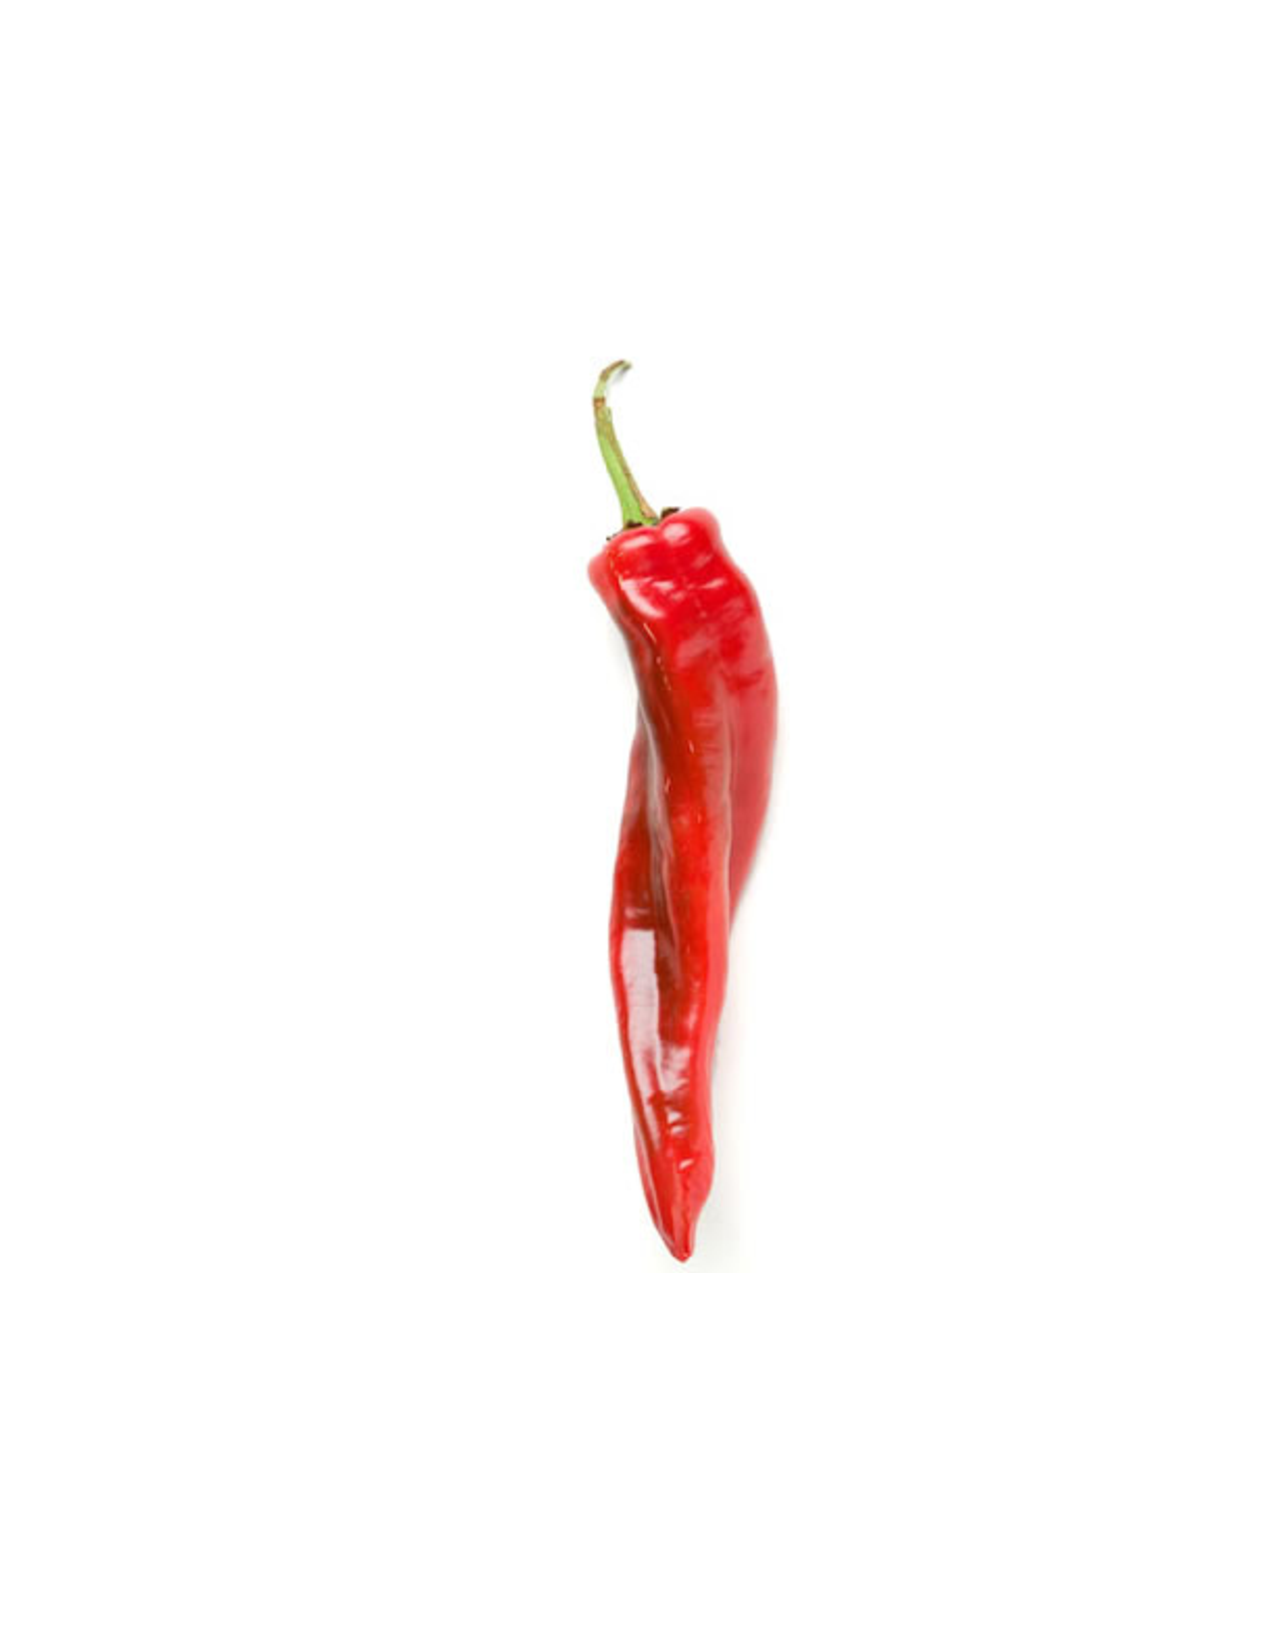
\includegraphics{figures/chili.pdf}}}
\newcommand{\chchili}{{\chili\chili}}
\newcommand{\chchchili}{{\chchili\chili}}

% The units package provides nice, non-stacked fractions and better spacing
% for units.
\usepackage{units}

% The fancyvrb package lets us customize the formatting of verbatim
% environments.  We use a slightly smaller font.
\usepackage{fancyvrb}
\fvset{fontsize=\normalsize}

% Small sections of multiple columns
\usepackage{multicol}

\hypersetup{
urlcolor=blue,
colorlinks=true
}
\usepackage[noline, procnumbered, linesnumberedhidden, boxed]{algorithm2e}

\newcommand{\openepigraph}[2]{ % This block sets up a command for printing an epigraph with 2 arguments - the quote and the author
\begin{fullwidth}
\sffamily\large
\begin{doublespace}
\noindent\allcaps{#1}\\ % The quote
\noindent\allcaps{#2} % The author
\end{doublespace}
\end{fullwidth}
}

\newcommand{\figref}[1]{Figure~\ref{#1}}
\renewcommand{\thefigure}{\arabic{figure}}

\newenvironment{callout}[1]{
\[
  \left[
      \begin{tabular}{@{\quad}m{.05\textwidth}@{\qquad}m{.75\textwidth}@{\quad}}
        \scalebox{1.5}{#1} & 
          \raggedright%
}
{
      \end{tabular}
    \right]
\]
}

\newcommand{\blankpage}{\newpage\hbox{}\thispagestyle{empty}\newpage} % Command to insert a blank page

\usepackage{makeidx} % Used to generate the index
\makeindex % Generate the index which is printed at the end of the document

\renewcommand{\maketitlepage}[0]{%
  \cleardoublepage%
  {%
  \sffamily%
  \begin{fullwidth}%
  ~
  \vspace{11.5pc}%
  \fontsize{36}{40}\selectfont\par\noindent\textcolor{darkgray}{\allcaps{\thanklesstitle}}%
  
\scalebox{.2}{
\includegraphics{figures/msan-logo}}
  \vspace{11.5pc}%
  \fontsize{12}{18}\selectfont\par\indent\textcolor{darkgray}{\allcaps{\thanklessauthor}\\
\indent{\tt parrt@cs.usfca.edu}\\
\href{http://parrt.cs.usfca.edu}{http://parrt.cs.usfca.edu}}%
  \vspace{11.5pc}%
  \fontsize{14}{16}\selectfont\par\noindent\allcaps{\thanklesspublisher}%
  \end{fullwidth}%
  }
  \thispagestyle{empty}%
  \clearpage%
}

\titlecontents{part}% FIXME
    [0em] % distance from left margin
    {\vspace{1.5\baselineskip}\begin{fullwidth}\LARGE\rmfamily\itshape} % above (global formatting of entry)
    {\contentslabel{2em}} % before w/label (label = ``II'')
    {} % before w/o label
    {\rmfamily\upshape\qquad\thecontentspage} % filler + page (leaders and page num)
    [\end{fullwidth}] % after

  \titlecontents{chapter}%
    [0em] % distance from left margin
    {\vspace{1.5\baselineskip}\begin{fullwidth}\Large\rmfamily\itshape} % above (global formatting of entry)
    {\hspace*{0em}\contentslabel{2em}} % before w/label (label = ``2'')
    {\hspace*{4em}} % before w/o label
    {\rmfamily\upshape\qquad\thecontentspage} % filler + page (leaders and page num)
    [\end{fullwidth}] % after

\titlespacing*{\chapter}{0pt}{0pt}{30pt}
\titlespacing*{\section}{0pt}{3.5ex plus 1ex minus .2ex}{2.3ex plus .2ex}
\titlespacing*{\subsection}{0pt}{3.25ex plus 1ex minus .2ex}{1.5ex plus.2ex}

\begin{document}

\chapter{Confidence Intervals for Price of Hostess Twinkies}

\setcounter{problem}{1}
\section{Goal}

\begin{fullwidth}


The goal of this project is to learn how to compute an empirical 95\% confidence interval for the sample mean price for Hostess Twinkies using an awesome technique called {\em bootstrapping}. Bootstrapping allows us to assess the accuracy of a sample mean we've computed, giving us data about how sample means vary. As part of this lab, you will also learn to read in a file full of numbers. In this case, we are going to read in the price of Hostess Twinkies, a tasty snack recently returned from the dead, from around the US.

\section{Discussion}

A sample mean confidence interval of 95\% tells us the range in which most (95\% or $1.96\sigma$) of the sample means fall.  All we have to do is create a number of samples, $X$, and compute the means $\overline{X}$.  If we do this lots of times (trials) then 95\% of the time, we would expect the sample mean to fall within the range of 95\% of the samples. We just have to order the $\overline{X}$ values and strip off the lower and top 2.5\%. Then, the lowest and highest value in that stripped list represent the boundaries of the confidence interval. Cool, right?

From the central limit theorem, we know that the distribution of $\overline{X}$ is $N(\overline{X}, \sigma^2/n)$ for sample size $n$ (not the number of trials). In this case, however, we don't know what the underlying distribution is because we just got a bunch of prices from a file. We could assume that it's normally distributed, but there's no point. The central limit theorem works on any underlying distribution we care about here but we do need the variance. For that, we can use the sample variance as an estimate of the variation in the overall Hostess Twinkies price population.  

The question is how do we get lots of trials from an underlying distribution that we cannot identify? By repeated sampling from our single sample {\em with replacement}. This is called {\em bootstrapping}, which you could also call {\em resampling}. The idea is to randomly select $N$ values from our known data set of size $N$. That gives us one trial. We can then repeatedly compute our test statistic, the mean, on each sample.

To verify that we are doing the right thing, we will draw the theoretical normal distribution expected by the Central limit theorem and then shade in the 95\% theoretical confidence interval, which we know is 1.96 standard deviations on either side of the mean: $\mu \pm 1.96\sigma$.

Please do your work in filename {\tt stats/conf.py}.

\section{Steps}

\step First, we have to get the data from a file called {\tt prices.txt} from \\
{\tt\small https://github.com/parrt/msan501/tree/master/data}:

\begin{pyverbatim}
prices = []
f = open("prices.txt")
for line in f:
	v = float(line.strip())
	prices.append(v)
\end{pyverbatim}

When debugging or during development, you can print those numbers out to verify they look okay.

\step Now, we need a function that lets us sample {\em with replacement} from that raw data set. In other words, we need a function that gets $n$ values at random from a data parameter (a list of numbers). It should allow repeated grabbing of the same value (that's what we call with replacement).

\begin{pyverbatim}
def sample(data):
	"""
	Return a random sample of data values with replacement.
	The returned array has same length as data.
	"""
\end{pyverbatim}

The idea is to get an array of random numbers from $U(0,n)$ for {\tt n=len(data)}. These then are a set of indices into the data array so just loop through this index array grabbing values from data according to the index. For example if you have indexes = [3,9] for a 2-element data array, then return a new array [data[3], data[9]. My solution has two lines in it.

\step Now define TRIALS=20 and perform that many samplings of prices. For each sample, create the sample mean and add it to an X\_ list.

\step Sort that list and get the values from indices TRIALS*0.025..TRIALS*0.975 in X\_ and call it {\tt inside}.

\step Print the first and last value of the {\tt inside} array as that will tell you what the bounds of your 95\% confidence interval are

\begin{pyverbatim}
print inside[0], inside[-1]
\end{pyverbatim}

\noindent 5\% of 40 is 2 which means grab 1 element on either side. You might get something like (there will be a lot of variation):

1.1270115942 1.17842898551

\step Add code to plot diamonds on the graph at those locations.

\step Now plot the normal curve using your amazing understanding of the central limit  theorem. Use the following range and also set the overall graph range:

\begin{pyverbatim}
x = np.arange(1.05, 1.25, 0.001)
plt.axis([1.10, 1.201, 0, 30])
x = np.arange(1.05, 1.25, 0.001)
y = stats.norm.pdf(x,mean,stddev)  # WHAT ARE MEAN AND STDDEV?
plt.plot(x,y, color='red')
\end{pyverbatim}

\step Run it and you should get the following graph:

\scalebox{.4}{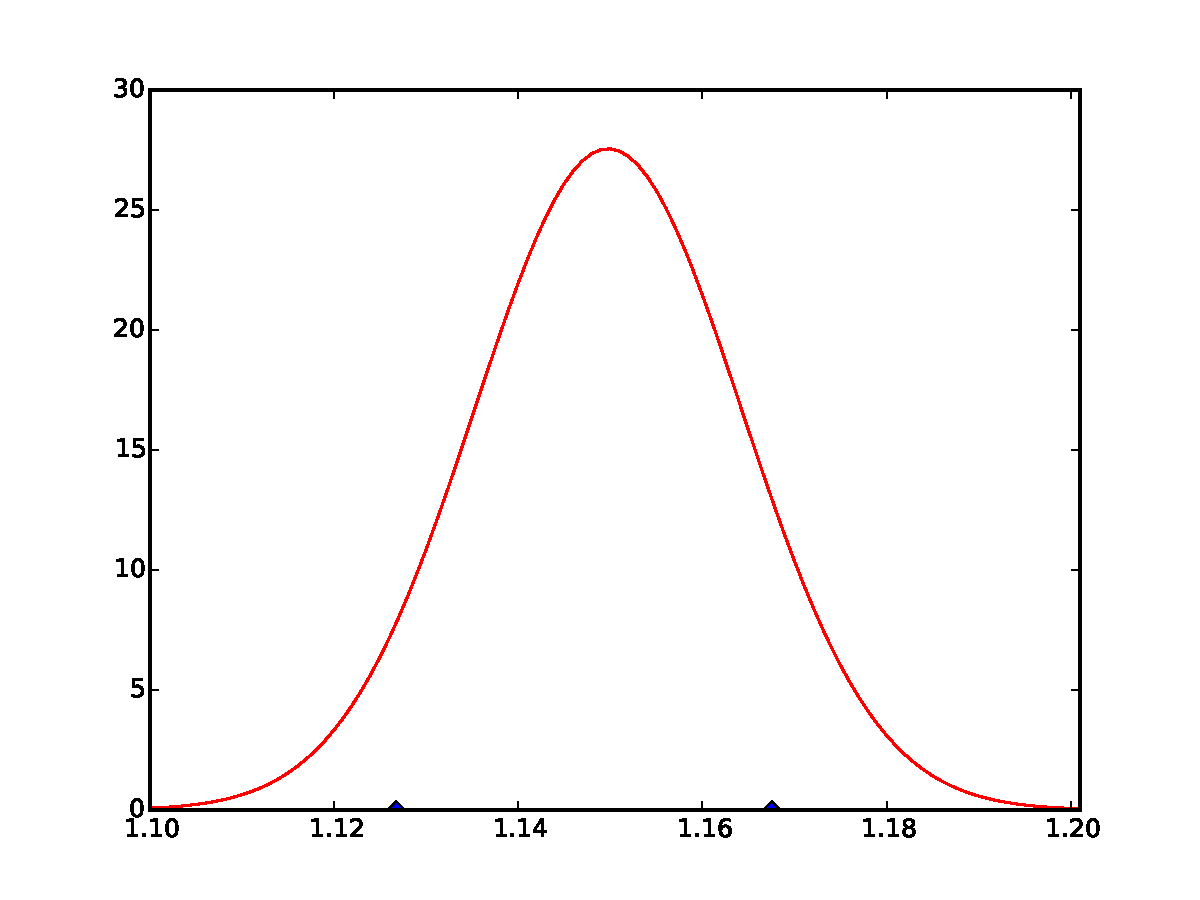
\includegraphics{figures/conf-40-basic.pdf}}

Ok, that's great but we have no idea if this is correct or not. Now, let's go nuts and show lots of stuff on the graph.

\step First, let's shade in the theoretical 95\% confidence interval using a function called {\tt normpdf()} that you implement from the symbolic definition of the normal density function:

\[
normpdf(x) = \frac{1}{{\sigma \sqrt {2\pi } }}e^{{{ - \left( {x - \mu } \right)^2 } \mathord{\left/ {\vphantom {{ - \left( {x - \mu } \right)^2 } {2\sigma ^2 }}} \right. \kern-\nulldelimiterspace} {2\sigma ^2 }}}
\]


\begin{pyverbatim}
def normpdf(x, mu, sigma):
    return ...

mean = ...
stddev = ...
# redraw normal but only shade in 95% CI
left  = ...
right = ...

ci_x = np.arange(left, right, 0.001)
ci_y = normpdf(ci_x,mean,stddev)
# shade under (ci_x,ci_y) curve
plt.fill_between(ci_x,ci_y,color="#F8ECE0") 
\end{pyverbatim}

\noindent Run it again to see how it shades in the graph.

\scalebox{.4}{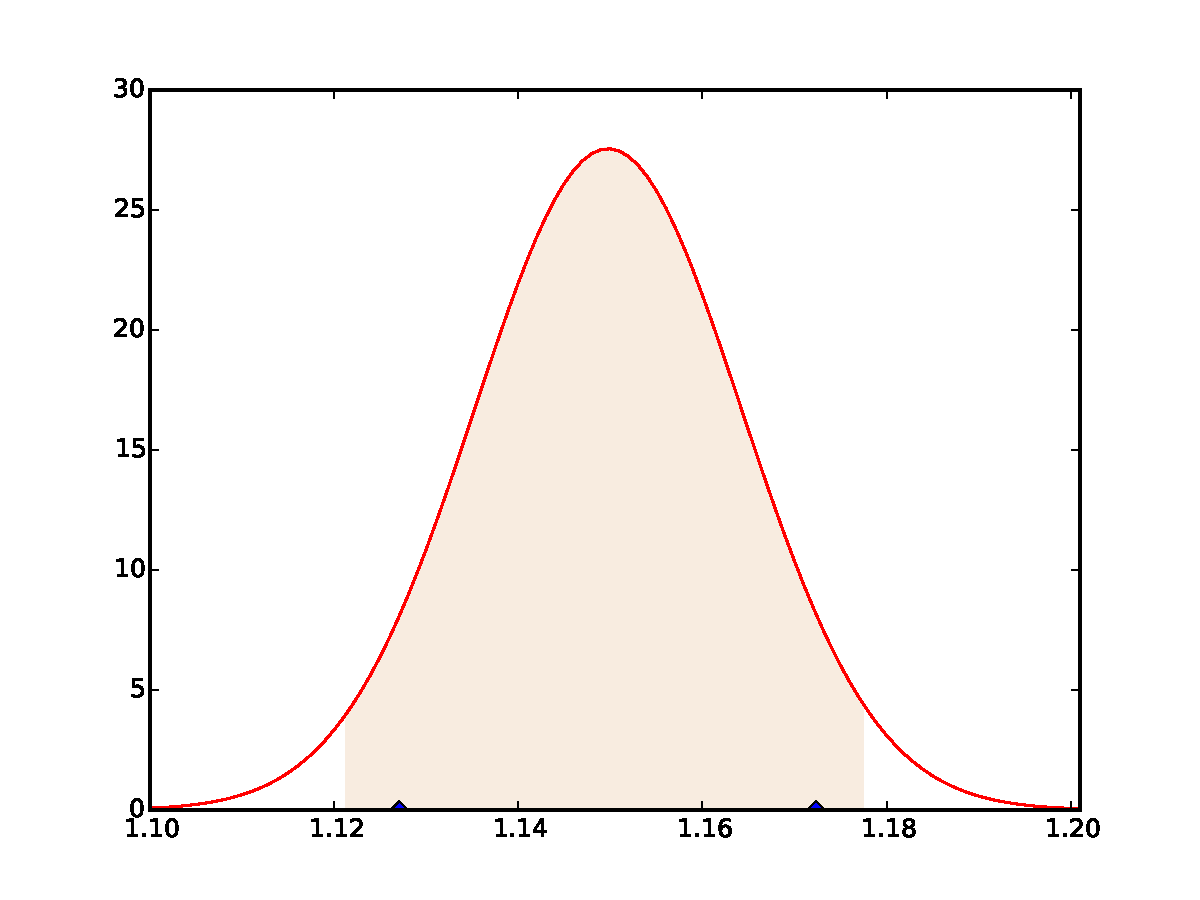
\includegraphics{figures/conf-40-noannot.pdf}}

\step Now let's annotate with lots of information. Please read through and figure out what all of that stuff does to draw the nice arrows and so on.

{\small
\begin{pyverbatim}
plt.text(.02,.95, '$TRIALS = %d$' % TRIALS, transform = ax.transAxes)
plt.text(.02,.9,  '$mean(prices)$ = %f' % np.mean(prices), transform = ax.transAxes)
plt.text(.02,.85, '$mean(\\overline{X})$ = %f' % np.mean(X_), transform = ax.transAxes)
plt.text(.02,.80, '$stddev(\\overline{X})$ = %f' %
    np.std(X_,ddof=1), transform = ax.transAxes)
plt.text(.02,.75, '95%% CI = $%1.2f \\pm 1.96*%1.3f$' %
   (np.mean(X_),np.std(X_,ddof=1)), transform = ax.transAxes)
plt.text(.02,.70, '95%% CI = ($%1.2f,\\ %1.2f$)' %
				  (np.mean(X_)-1.96*np.std(X_),
				   np.mean(X_)+1.96*np.std(X_)),
		 transform = ax.transAxes)

plt.text(1.135, 11.5, "Expected", fontsize=16)
plt.text(1.135, 10, "95% CI $\\mu \\pm 1.96\\sigma$", fontsize=16)
plt.title("95% Confidence Intervals: $\\mu \\pm 1.96\\sigma$", fontsize=16)

ax.annotate("Empirical 95% CI",
			 xy=(inside[0], .3),
			 xycoords="data",
			 xytext=(1.13,4), textcoords='data',
			 arrowprops=dict(arrowstyle="->",
                            connectionstyle="arc3"),
			 fontsize=16)
\end{pyverbatim}
}

\step Run it and you should get the following graph:

\scalebox{.4}{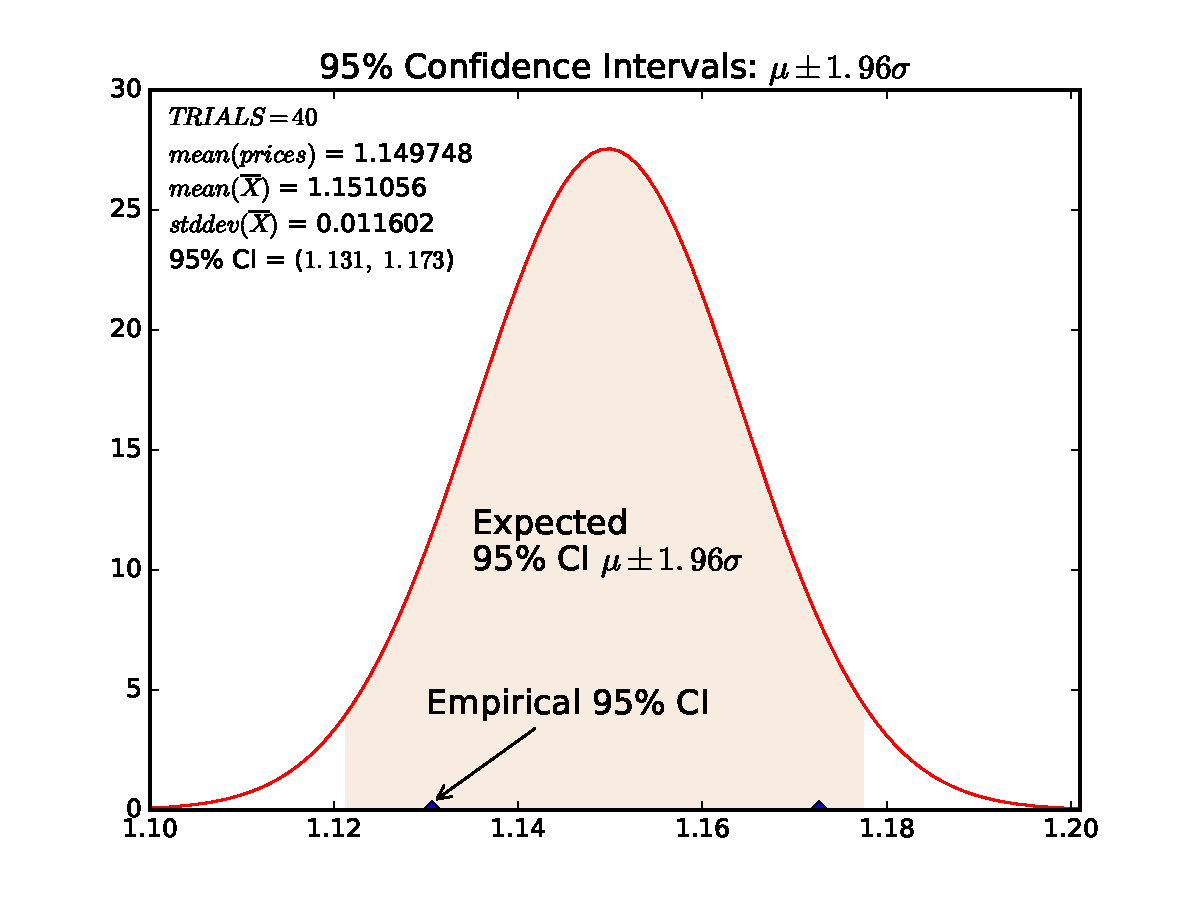
\includegraphics{figures/conf-40.pdf}}

\step We need to make the number of trials a parameter and let's do the annotations as well.  

\begin{pyverbatim}
import sys

fancy=False
TRIALS = 40
if len(sys.argv)>1:
    TRIALS = int(sys.argv[1])
    if len(sys.argv)>2 and sys.argv[2]=='-fancy':
        fancy=True
\end{pyverbatim}

\noindent Then wrap your annotation code in {\tt if fancy} and add code to save your graph (in all cases):

\begin{pyverbatim}
plt.savefig('conf-'+str(TRIALS)+('-basic' if not fancy else '')+'.pdf', format="pdf")
\end{pyverbatim}

\step  We don't have to increase the number of trials very much before the confidence interval tightens up nicely. Try 500:

\begin{alltt}
$ python conf.py 500 -fancy
\end{alltt}

\noindent You'll get:

\scalebox{.4}{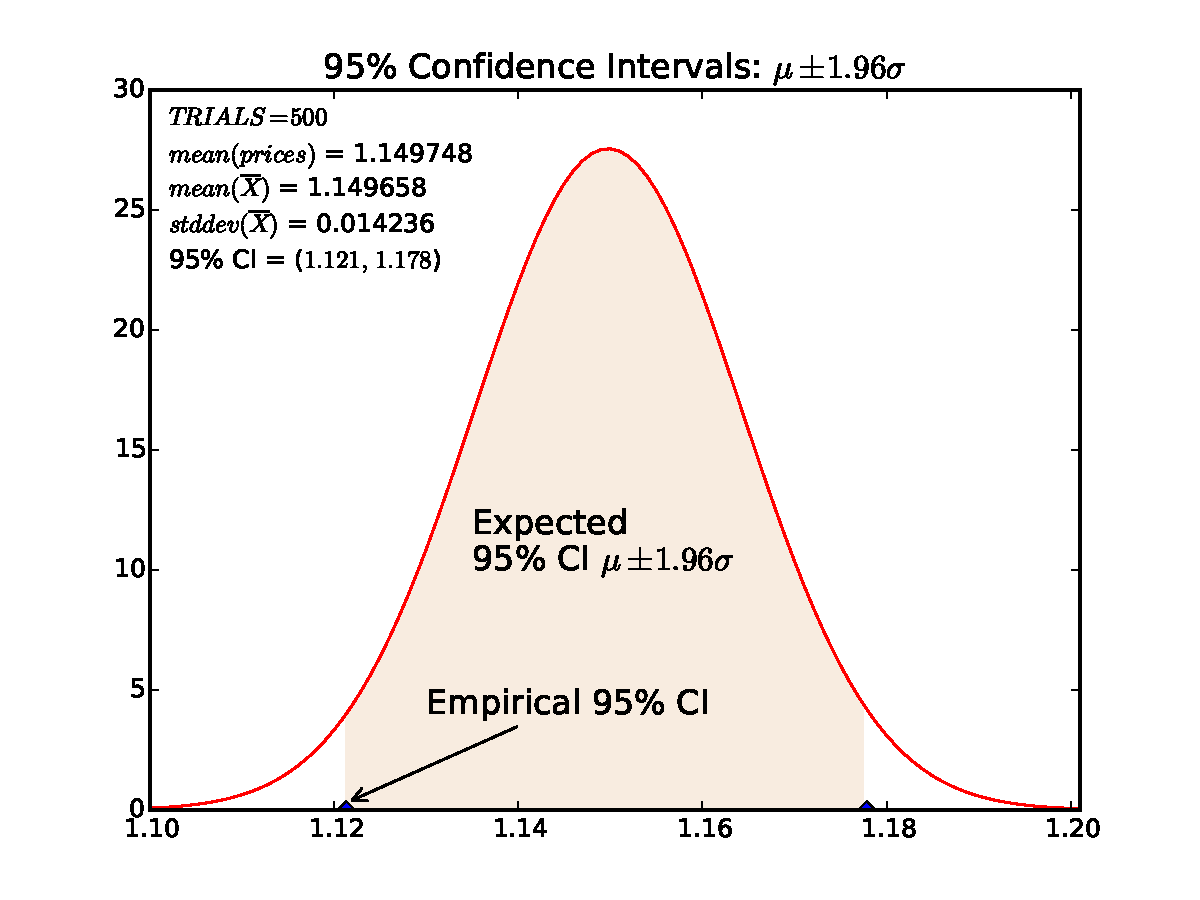
\includegraphics{figures/conf-500.pdf}}

\begin{callout}{\bcplume}
{\bf Deliverables}. {\tt stats/conf.py} and a PDF called {\tt conf-500.pdf}, the result of $TRIALS=500$.
\end{callout}

\end{fullwidth}

\end{document}